\documentclass[referee]{gji}
\usepackage{timet,color}
\usepackage{graphicx}
\usepackage{amsmath}
\usepackage{amssymb}
\usepackage{booktabs}
\usepackage{longtable}
\usepackage{url}
\usepackage[switch]{lineno}
\makeatletter
\let\bibhang\relax
\makeatother
\usepackage{gji_extra}
\usepackage[hidelinks]{hyperref}
\newcommand{\figalt}[1]{}

\title[Audited probabilistic surface-wave inversion]
  {Auditing Learned Posterior Samples for Surface-Wave Dispersion Inversion}

\author[X. Liu et al.]
  {Xin Liu$^1$, Ziye Yu$^1$\thanks{Corresponding author: yuziye@cea-igp.ac.cn}
  and Yuqi Cai$^1$\\
  $^1$Institute of Geophysics, China Earthquake Administration, Beijing 100081, China
  }

\date{}
\pagerange{\pageref{firstpage}--\pageref{lastpage}}
\volume{000}
\pubyear{2026}

\let\leqslant=\leq

\begin{document}
\label{firstpage}
\maketitle
\linenumbers
\pagestyle{plain}

\begin{summary}
Surface-wave dispersion inversion is non-unique, so a useful inverse method should report both a preferred model and the uncertainty attached to it. Bayesian inversions and earlier probabilistic neural networks already provide posterior distributions, but a learned posterior is only meaningful relative to the prior, forward solver, data mask, noise assumption and parameterisation used to train it. We develop a probabilistic direct-inversion (DI) method in which a depth-controlled conditional rectified flow generates ensembles of 1-D $V_P$, $V_S$ and density profiles for incomplete Rayleigh/Love phase-velocity curves, and we use the method to test how such learned posteriors can be audited.

Matched DI-Strong and DI-Weak models are trained from scratch with identical budgets so that only the structural prior differs. In the $N=1024$ inside-support diagnostic, DI-Strong reaches posterior-median $V_S$ mean absolute error (MAE) of 0.086 km s$^{-1}$ and mean pointwise 16--84 per cent interval coverage of 0.638. The prior-support test shows the expected trade-off: DI-Weak reduces near-edge and outside-support $V_S$ MAE to 0.171 and 0.499 km s$^{-1}$, compared with 0.372 and 0.782 km s$^{-1}$ for DI-Strong, while losing inside-support accuracy. On a same-site CSRM common-input benchmark using Rayleigh fundamental-mode phase velocities at 8--60 s, DI-Strong reaches mean $V_S$ MAE of 0.108 km s$^{-1}$, comparable to QEDisp fundamental-mode multistart inversion (0.104 km s$^{-1}$) and DispFormer phase-only prediction (0.111 km s$^{-1}$). Split-sample posterior-temperature scaling improves held-out mean coverage but is only a calibration check, not an observational likelihood. These results support a conservative interpretation: the proposed sampler is competitive as a point estimator, but its main value is that posterior samples, prior support, coverage, missing-band behaviour and noise sensitivity can be checked explicitly.
\end{summary}

\begin{keywords}
Inverse theory -- Probability distributions -- Neural networks -- Surface waves and free oscillations -- Seismic velocities -- Computational seismology.
\end{keywords}

\section{Introduction}

Geophysical inverse problems are rarely one-to-one. Surface-wave dispersion curves constrain weighted averages of elastic structure over period-dependent depth ranges, and many velocity models can explain similar observations. Classical inverse-problem theory therefore treats the answer as a posterior probability distribution rather than as a single preferred model \citep{MosegaardTarantola1995,Tarantola2005}. In surface-wave applications, stochastic and transdimensional methods have made this non-uniqueness explicit by mapping trade-offs among layer velocities, discontinuity depths, smoothing assumptions and data errors \citep{Sambridge1999,ShapiroRitzwoller2002,BodinEtAl2012,GaoLekic2018}. A useful inversion method should therefore report not only a central model but also uncertainty summaries that can be checked against known synthetic truth or independent constraints.

Conventional surface-wave inversions handle this ambiguity through regularisation, multiple initial models or stochastic searches, but these choices bring their own dependence on parameterisation and starting models. Recent physics-based software has improved this workflow. For example, QEDispInv improves modal dispersion calculation in low-velocity-layered models and combines wavelength-constrained layering with multiple initial models to reduce local-solution bias \citep{PanEtAl2026QEDispInv}. Such methods provide an important baseline because they keep the forward physics explicit, but their cost still grows with the number of sites, starts and posterior checks.

The same cost motivates learned inversion. A deep neural network (DNN) can be trained on synthetic pairs of Earth models and dispersion curves, and then used as a fast inverse map. Early neural approaches estimated crustal thickness or velocity-model uncertainty from surface waves \citep{DevileeEtAl1999,MeierEtAl2007}, and later networks extended learned inversion to near-surface, regional and uncertainty-aware settings \citep{HuEtAl2020,EarpEtAl2020,YablokovEtAl2021,YablokovEtAl2023,KeilWassermann2023,ChenEtAl2022,LuoEtAl2022}. Invertible neural networks have also been used to approximate Bayesian posteriors for surface-wave dispersion and related geophysical inverse problems \citep{ZhangCurtis2021}. These studies show that neural networks can predict models quickly and can, in some settings, approximate uncertain inverse solutions. The remaining issue addressed here is how to check the reliability of a posterior returned by a synthetic-trained DNN.

Large public data products and pretrained models are also changing the reference point for this field. OpenSWI provides synthetic and real-world benchmark data for surface-wave inversion \citep{LiuEtAl2026OpenSWI}, while DispFormer uses a transformer architecture to handle Rayleigh phase and group curves with variable period ranges and missing values \citep{LiuEtAl2025DispFormer}. These advances are strong baselines for point prediction and generalisation. The present work has a different emphasis: it studies posterior sampling and posterior reliability under a documented training distribution, rather than variable-period foundation-model generalisation.

In this paper, learned inversion is treated as simulation-based inference: a prior generator and a forward simulator define a synthetic training problem, and the network learns an approximation to the corresponding conditional distribution \citep{CranmerEtAl2020}. In SBI terms, this is an amortized neural posterior estimation problem: the expensive prior-predictive simulations are used during training, after which new dispersion inputs can be mapped rapidly to posterior samples. Ordinary deterministic DNN inversions tend to return point estimates and can hide the non-uniqueness that motivates Bayesian inversion in the first place. Our focus is on direct posterior sampling and reliability checks, not on replacing all conventional or pretrained point-estimation methods.

Conditional rectified flow offers a direct way to return samples rather than a single regressed profile. After training, different random initial states are mapped to different elastic structures conditioned on the same dispersion curve. The resulting ensemble can be summarised by posterior medians, pointwise 16--84 per cent intervals, posterior standard deviations and posterior density views. Those summaries are useful only if their calibration is tested, because a visually plausible ensemble can still be too narrow, too broad or biased by the training distribution.

The contribution of this study is a reliability-centred framework for a learned posterior sampler. Four elements are combined. The method returns posterior samples rather than only one regressed model. It samples a compact set of depth controls and evaluates the result on the full depth grid. It checks the samples with surface-wave quantities, including dispersion residuals, depth-binned coverage and rank diagnostics. It also keeps the training prior, forward solver and data mask explicit, so that the reported uncertainty can be tied back to the synthetic inversion problem.

This paper develops a probabilistic direct-inversion (DI) method based on a depth-controlled conditional rectified flow. The method learns $q_\theta({\bf m}|{\bf d})$, a distribution of 1-D elastic models ${\bf m}$ conditioned on a masked Rayleigh/Love dispersion vector ${\bf d}$. We ask four questions. First, what range of models does a DNN learn from synthetic model--dispersion pairs? Second, can a depth-controlled conditional flow produce regular posterior samples while preserving full-grid evaluation? Third, can posterior uncertainty be checked with empirical coverage and calibration diagnostics? Fourth, how sensitive is the learned posterior to prior support?

The central result is that a depth-controlled conditional rectified flow can provide fast posterior ensembles for surface-wave dispersion, but those ensembles must be read together with the training assumptions. In this setting the prior is encoded by the synthetic model generator, velocity and density bounds, depth clipping, layer or control-point parameterisation, wave-type availability, observation masks and noise augmentation. Figure~\ref{fig:workflow} summarizes this idea. We therefore include a matched prior-support test comparing strong- and weak-prior samplers trained with the same budget, missing-band and noise-sensitivity checks, posterior-temperature calibration, and a same-site external benchmark against QEDisp and DispFormer under a common Rayleigh-phase input. The aim is to show how DNN posterior uncertainty can be sampled, compared with established inversions and then audited within a clearly defined synthetic inversion problem.

\section{Bayesian target and synthetic training distribution}

\subsection{Bayesian object learned by the DNN}

Let ${\bf m}$ denote the 1-D model state and ${\bf d}$ the dispersion observation. The formal Bayesian target is
\begin{equation}
p({\bf m}|{\bf d}) \propto p({\bf d}|{\bf m})p({\bf m}),
\label{eq:bayes}
\end{equation}
but the DNN does not evaluate this expression analytically during inference. Instead, it is trained on synthetic pairs generated by
\begin{equation}
\begin{split}
{\bf m}&\sim p_{\rm syn}({\bf m}),\qquad
{\bf q}\sim p_{\rm mask}({\bf q}),\\
{\bf d}&=\mathcal{E}_{\bf q}\left[\mathcal{F}({\bf m})+\boldsymbol{\epsilon}\right],
\qquad
\boldsymbol{\epsilon}\sim p_\epsilon .
\end{split}
\label{eq:priorpredictive}
\end{equation}
Here $p_{\rm syn}$ is the synthetic structural prior, $\mathcal{F}$ is the Rayleigh/Love forward solver, ${\bf q}$ is the observation mask, $\mathcal{E}_{\bf q}$ encodes the masked data vector and $p_\epsilon$ is the assumed synthetic observation-error distribution. In the present benchmark no additive phase-velocity noise is applied, so $p_\epsilon$ is a point mass at zero and the stochastic observation process is the masking operation. These choices define the synthetic population $p_{\rm train}({\bf m},{\bf d})$ and the target conditional distribution $p_{\rm train}({\bf m}|{\bf d})$. The DNN learns an approximation $q_\theta({\bf m}|{\bf d})$ to that distribution.

Throughout this paper, posterior probability means probability for this stated synthetic inversion problem. It is not a calibrated posterior for arbitrary field dispersion measurements unless the field data are represented by a suitable observational-error model and the posterior is independently calibrated. This distinction is the reason for treating training-prior support as a reliability check rather than as a hidden data-generation detail.

\begin{figure*}[t]
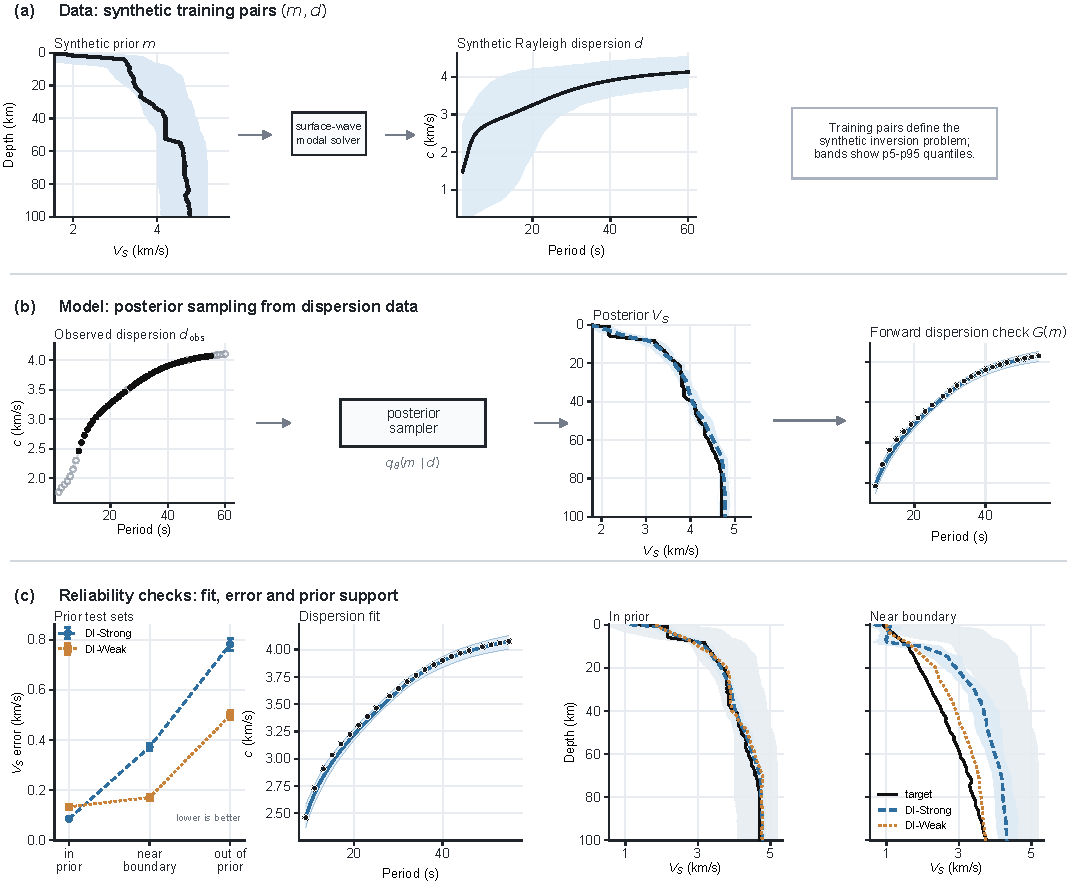
\includegraphics[width=\textwidth]{figures/fig01_workflow_prior_posterior_audit_p5p95.pdf}
\caption{Probabilistic direct inversion with prior checks. (a) Synthetic training pairs are generated by drawing elastic Earth models from a structural prior and computing Rayleigh dispersion with a surface-wave modal solver. Shaded bands show p5--p95 sample quantiles of the synthetic model and dispersion distributions, not observational-error bars. (b) The conditional-flow sampler takes an observed or masked dispersion curve and returns an ensemble of plausible $V_S$ profiles. The samples can be forward-modelled to check whether they reproduce the input dispersion. (c) Reliability checks compare matched DI-Strong and DI-Weak samplers on inside-support, near-edge and outside-support test sets. The profile panels show representative inside-support and near-edge cases; shaded posterior bands are p5--p95 pointwise sample quantiles. Coverage values elsewhere in the paper are computed separately for 16--84 per cent intervals.}
\figalt{Three-row method diagram showing synthetic model--dispersion pair generation, conditional-flow posterior sampling with dispersion checking, and reliability checks across inside-support, near-edge and outside-support test sets.}
\label{fig:workflow}
\end{figure*}

\subsection{Diagnostic weak-prior generator}

The weak-prior diagnostic sampler uses a broad structural prior. This generator uses broad depth-dependent bounds rather than explicit tectonic classes, Moho templates or prescribed low-velocity-zone forms. It expands admissible ranges for $V_P$, $V_S$, density, sediment thickness, Moho depth, upper-mantle velocity, and low-velocity-zone depth and amplitude while retaining physical constraints such as $V_P>V_S$, positive $V_S$ and reasonable density. Random control points and weakly correlated perturbations allow a wider family of smooth profiles.

The weak prior is not prior-free. It still imposes velocity bounds, smoothness preferences, physical consistency rules and a depth basis. Its purpose is to make the learned posterior less dependent on narrow tectonic templates and less likely to exclude plausible structures before inversion. Because the same dispersion observation is compatible with a broader set of models, a weak-prior posterior should also be broader and harder to learn from finite training data. This is the intended trade-off tested below.

\subsection{Strong structural prior as a narrow-prior control}

The strong-prior control is generated from a synthetic 1-D tectonic model prior. Each sample contains depth, $V_P$, $V_S$ and density on a regular 0.5 km grid. Five broad tectonic classes are sampled: oceanic, shield, platform, orogen and rift. Each class defines ranges for crustal thickness, sediment thickness, upper- and lower-crustal $V_S$, upper-mantle $V_S$, and the probability, depth and amplitude of an upper-mantle low-velocity zone. $V_P$ is generated from layer-dependent $V_P/V_S$ ratios, and density is computed from empirical crustal relations \citep{Brocher2005}. This prior is geologically structured and useful for stabilising inversion, but it is deliberately bounded. We use it to quantify what is gained and lost when the direct posterior sampler is trained on a narrow prior.

Appendix Table~\ref{tab:priorparameters} lists the main parameter ranges used by the two generators. These values are not fitted to the field data in this manuscript; they define the synthetic inversion problem used to train and test $q_\theta({\bf m}|{\bf d})$.

For both priors, the full model vector is
\begin{equation}
{\bf m}(z)=\{V_P(z),V_S(z),\rho(z)\},
\end{equation}
sampled at 256 depth nodes, giving a maximum represented depth of 127.5 km. The depth coordinate is fixed. Surface-wave phase velocities are computed for periods from 2 to 60 s using a Python implementation of surface-wave dispersion routines based on Computer Programs in Seismology \citep{Herrmann2013,LuuDisba}. The observation vector contains normalised period, Rayleigh velocity, Love velocity and separate masks for the two wave types. Missing velocities are set to zero after normalisation and are identified by the masks.

\subsection{Depth-control representation}

Although the posterior is evaluated on the full 256-node grid, the DNN samples values at 28 depth controls and then linearly interpolates to the full grid. Weak-prior ensemble summaries and the 28-control basis are shown in Fig.~\ref{fig:controlpoints}. The controls are dense near the surface and sparse at depth: 0--5 km every 0.5 km, 5--10 km every 1 km, 10--50 km every 5 km and 50--127.5 km every 20 km. Let ${\bf m}_{\rm cp}$ be the vector of $V_P$, $V_S$ and density at these control depths. The full profile is
\begin{equation}
{\bf m}(z_i)=\mathcal{I}\left[{\bf m}_{\rm cp}\right](z_i),
\end{equation}
where $\mathcal{I}$ is a fixed differentiable interpolation operator. This basis is part of the training problem because it restricts the stochastic degrees of freedom available to the posterior sampler.

\begin{figure*}
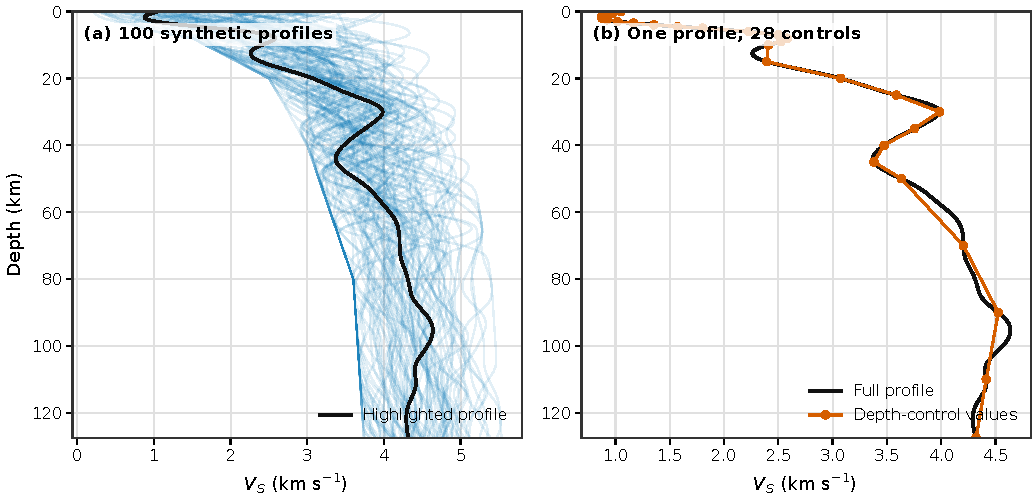
\includegraphics[width=\textwidth]{figures/fig02_control_points.pdf}
\caption{Weak-prior $V_S$ ensemble summary and depth-control basis. (a) Pointwise 10--90 per cent range and median profile from weak-prior samples. (b) Median $V_S$ control values at 28 nonuniform depths, linearly interpolated to the 256-node grid used for training losses and posterior summaries.}
\figalt{Two-panel figure showing the weak-prior shear-velocity envelope and the 28-control interpolation basis used to represent full-grid profiles.}
\label{fig:controlpoints}
\end{figure*}

\section{DNN posterior sampler}

\subsection{Conditioning encoder}

The conditional input has five period-indexed channels: normalised period, normalised Rayleigh phase velocity, normalised Love phase velocity, Rayleigh mask and Love mask. A one-dimensional convolutional encoder with residual blocks maps this input to a 256-dimensional conditioning vector. The encoder sees both measured velocities and the pattern of missing observations, so the posterior sampler can represent cases with Rayleigh only, Love only, both wave types or incomplete period windows. In the present implementation these incomplete observations are represented on a fixed 2--60 s period grid. The masks emulate missing or quality-controlled picks within that grid; they should not be interpreted as unrestricted variable-period generalisation.

\subsection{Conditional rectified flow}

The depth-control target ${\bf m}_{\rm cp}$ is normalised by the training-set mean and standard deviation to form ${\bf z}_{\rm cp}$. During training, a Gaussian sample $\boldsymbol{\epsilon}\sim N(0,I)$ and a time $t\sim U(0,1)$ define the straight-line interpolation
\begin{equation}
{\bf x}_t=(1-t)\boldsymbol{\epsilon}+t{\bf z}_{\rm cp}.
\end{equation}
The velocity field $v_\theta({\bf x}_t,t,{\bf d})$ is trained to predict the displacement from noise to target:
\begin{equation}
\mathcal{L}_{\rm flow}=
\mathbb{E}\left[
\left\|v_\theta({\bf x}_t,t,{\bf d})-({\bf z}_{\rm cp}-\boldsymbol{\epsilon})\right\|_1
\right],
\label{eq:flowloss}
\end{equation}
implemented with a SmoothL1 loss. A one-step reconstruction term evaluates
\begin{equation}
\widehat{\bf z}_{\rm cp}={\bf x}_t+(1-t)v_\theta({\bf x}_t,t,{\bf d})
\end{equation}
and adds small first- and second-difference penalties after interpolation to the full depth grid. This encourages physically smooth posterior draws without post-processing the final samples.

After training, sampling starts from ${\bf x}_0\sim N(0,I)$ and integrates
\begin{equation}
\frac{d{\bf x}_t}{dt}=v_\theta({\bf x}_t,t,{\bf d})
\label{eq:ode}
\end{equation}
from $t=0$ to $t=1$. The endpoint is denormalised in control-point space and interpolated to the full grid. The push-forward distribution of the Gaussian source through this conditional ordinary differential equation is the learned posterior approximation $q_\theta({\bf m}|{\bf d})$. Rectified flow and related continuous-flow models provide an efficient way to learn such transport maps \citep{LiuGongLiu2022,LipmanEtAl2023}; invertible neural networks have been used similarly for ambiguous inverse problems \citep{ArdizzoneEtAl2019}.

\subsection{Training and posterior summaries}

DI-Strong and DI-Weak are trained from scratch with matched budgets: 100000 synthetic profiles, 2048 validation profiles, batch size 64, 24 scheduled epochs, the same encoder and conditional-flow architecture, the same optimizer and learning-rate schedule, the same loss weights, the same intermittent-band mask augmentation and the same random seed. The analysed checkpoint for each run is selected by validation total loss. The only intended difference is the structural prior generator. Unless otherwise stated, posterior summaries use 64 samples and 24 Euler steps. Point estimates are posterior medians computed independently at each depth and parameter. Quantitative coverage diagnostics use pointwise marginal 16--84 per cent intervals from the sampled ensemble; figures that use wider p5--p95 bands are labelled accordingly.

Empirical coverage is computed pointwise over model parameters and depths:
\begin{equation}
C_{16-84}=
\frac{1}{3ND}
\sum_{n=1}^{N}
\sum_{c=1}^{3}
\sum_{i=1}^{D}
{\bf 1}\left[
q_{0.16,nci}\le m^{\rm true}_{nci}\le q_{0.84,nci}
\right],
\label{eq:coverage}
\end{equation}
where $N$ is the number of evaluation examples, $D=256$ is the number of depth samples, $c$ indexes $V_P$, $V_S$ and density, and $q_{0.16}$ and $q_{0.84}$ are posterior-sample quantiles. This is marginal pointwise coverage, not the probability that an entire profile lies inside the plotted band.

We also use a simple split-sample posterior-temperature diagnostic. For each posterior sample ${\bf m}_s$ and pointwise posterior median $\widetilde{\bf m}$, the scaled sample is
\begin{equation}
{\bf m}^{(\tau)}_s=
\widetilde{\bf m}+\tau({\bf m}_s-\widetilde{\bf m}).
\label{eq:temperature}
\end{equation}
The scalar $\tau$ is fitted on a calibration subset to make mean pointwise 16--84 per cent coverage close to the nominal 0.68 target and is then evaluated on a held-out subset. This operation widens or narrows intervals without changing posterior medians. It is a diagnostic of posterior dispersion, not a replacement for a physical observational-error likelihood. The production result tables report the fitted temperature factors and held-out reliability curves for all methods and regimes.

\subsection{Prior-boundary diagnostic}

The prior-support diagnostic changes the test distribution while keeping the forward solver and observation format fixed. Three regimes are used. The inside-support set contains models drawn from the strong-prior generator. The near-edge set places Moho depth, sediment thickness, upper-mantle $V_S$ and low-velocity-zone depth or amplitude close to the strong-prior limits. The outside-support set remains physically plausible but deliberately exceeds strong-prior support through thicker sediments, shifted Moho depths, stronger low-velocity zones, upper-mantle velocities outside default ranges or sharper gradients.

DI-Weak denotes the weak-prior conditional rectified-flow sampler and is the broad-prior configuration considered here. DI-Strong denotes the matched strong-prior sampler and is used as a narrow-prior control. Because DI-Strong and DI-Weak are trained with matched budgets, the numerical comparison isolates the structural-prior generator; it is a test of training-prior support rather than a universal prior ranking.

For each method and test regime we compute $V_P$, $V_S$ and density mean absolute error (MAE), root-mean-square error, posterior interval coverage, forward-modelled dispersion residual and a prior-support pull-in statistic. The pull-in statistic estimates a pointwise 1--99 per cent envelope from the strong-prior training distribution. It then measures the fraction of target values outside that envelope whose posterior median is returned inside the envelope. Large pull-in indicates that the direct posterior map is drawing unfamiliar structures back into the strong-prior support.

\section{Results}

\subsection{Deep-learning posterior sampling performance}

The matched inside-support diagnostics show that the depth-controlled conditional rectified flow returns useful model ensembles under both structural priors (Table~\ref{tab:validation}; Fig.~\ref{fig:directexamples}). DI-Strong has lower inside-support median error, with $V_S$ MAE of 0.086 km s$^{-1}$ and mean 16--84 per cent coverage of 0.638. DI-Weak has broader structural support but higher inside-support error, with $V_S$ MAE of 0.134 km s$^{-1}$ and mean coverage of 0.577. The lower $V_S$ error relative to $V_P$ and density is expected because fundamental-mode surface-wave dispersion is most directly sensitive to shear velocity; $V_P$ and density are recovered mainly through prior correlations and physical constraints encoded in the synthetic generator.

\begin{table*}
\caption{Matched inside-support diagnostic statistics for DI-Strong and DI-Weak trained from scratch with identical budgets. Posterior summaries use 64 samples and 24 Euler steps. Coverage is mean pointwise 16--84 per cent interval coverage over $V_P$, $V_S$ and density; bootstrap confidence intervals are reported in the CSV/JSON result tables.}
\label{tab:validation}
\centering
\begin{tabular}{@{}lccccc@{}}
\toprule
Method & $N$ & $V_P$ MAE & $V_S$ MAE & Density MAE & Coverage \\
 & & (km s$^{-1}$) & (km s$^{-1}$) & (g cm$^{-3}$) & \\
\midrule
DI-Strong & 1024 & 0.235 & 0.086 & 0.079 & 0.638 \\
DI-Weak & 1024 & 0.333 & 0.134 & 0.150 & 0.577 \\
\bottomrule
\end{tabular}
\end{table*}

\begin{figure*}
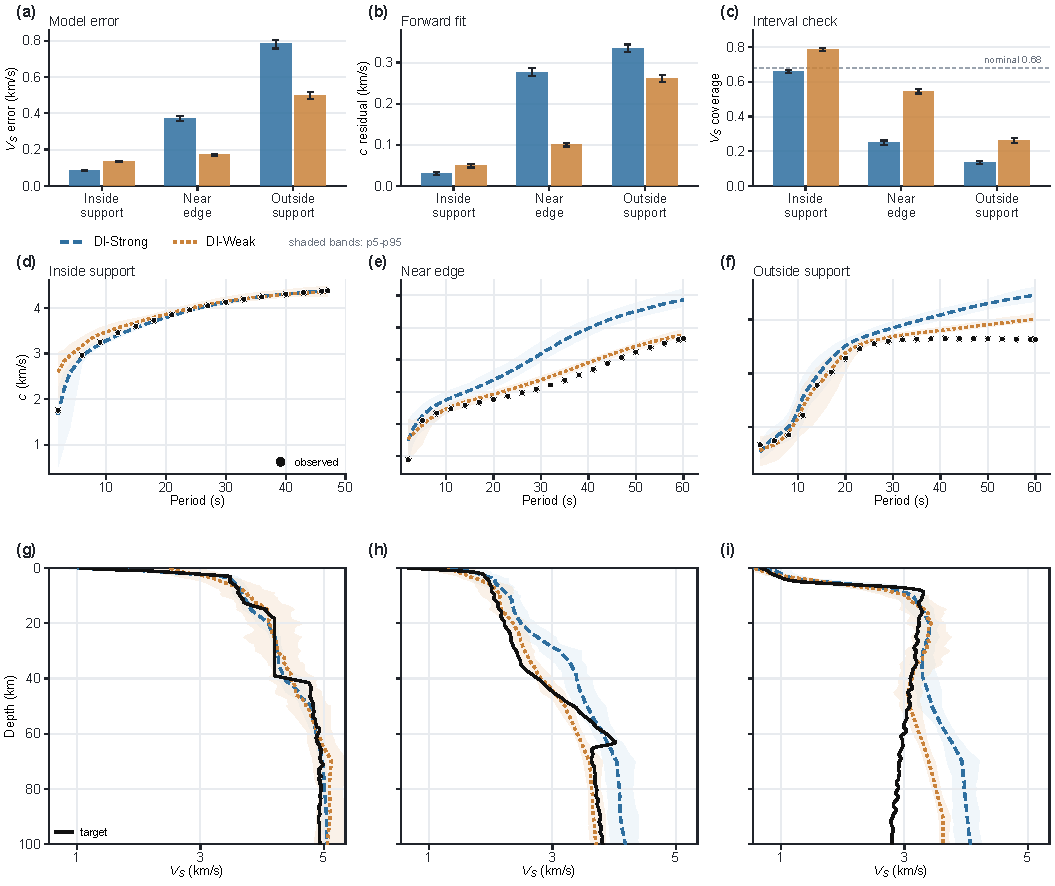
\includegraphics[width=\textwidth]{figures/fig03_direct_inversion_results_v9.pdf}
\caption{Matched production diagnostics for the conditional-flow posterior sampler. (a--c) $V_S$ model error, forward-modelled dispersion residual and empirical 16--84 per cent $V_S$ coverage for DI-Strong and DI-Weak on identical inside-support, near-edge and outside-support test sets. The dashed line in (c) marks nominal 0.68 coverage. (d--f) Representative Rayleigh dispersion fits obtained by forward-modelling posterior samples. (g--i) Corresponding $V_S$ profiles for the same examples. Black curves or points are the target model or observed dispersion; coloured curves show posterior medians; shaded bands show p5--p95 pointwise posterior-sample quantiles.}
\figalt{Nine-panel diagnostic figure comparing DI-Strong and DI-Weak across inside-support, near-edge and outside-support cases, with error bars, coverage bars, dispersion fits and shear-velocity posterior profiles.}
\label{fig:directexamples}
\end{figure*}

\subsection{Empirical coverage and posterior-temperature calibration}

Raw posterior intervals are informative but not automatically calibrated (Fig.~\ref{fig:coverage}). On the inside-support held-out split, raw 68 per cent mean coverage is 0.631 for DI-Strong and 0.580 for DI-Weak. Scalar posterior-temperature scaling fitted on a separate calibration half gives held-out mean coverage of 0.681 and 0.685, with temperature factors of 1.114 and 1.316, respectively. Near-edge and outside-support regimes require much larger corrections for DI-Strong ($\tau=3.160$ and 4.584), reflecting mismatch with the strong training prior. DI-Weak needs smaller near-edge correction ($\tau=1.687$) but still needs substantial outside-support widening ($\tau=3.335$). These results show that the DNN can return a spread of possible models, but that the nominal intervals must be checked before they are read as probabilities.

Depth-binned coverage and rank diagnostics tell the same story with more spatial detail. For inside-support DI-Strong, raw depth-binned 68 per cent coverage ranges from 0.588 to 0.752 across channel-depth bins and becomes 0.641--0.795 after temperature scaling. DI-Weak has a wider raw inside-support range, 0.205--0.860, which becomes 0.258--0.941 after scaling; this indicates that one scalar temperature corrects the mean interval width but does not remove all depth- and parameter-dependent miscalibration. Rank/probability-integral-transform (PIT) histograms are also non-uniform before scaling: the two edge bins contain 0.201 of inside-support DI-Strong ranks and 0.281 of inside-support DI-Weak ranks, compared with 0.10 for a uniform diagnostic. We therefore report both mean reliability curves and depth-binned/rank tables rather than relying on one aggregate coverage number.

\begin{figure}
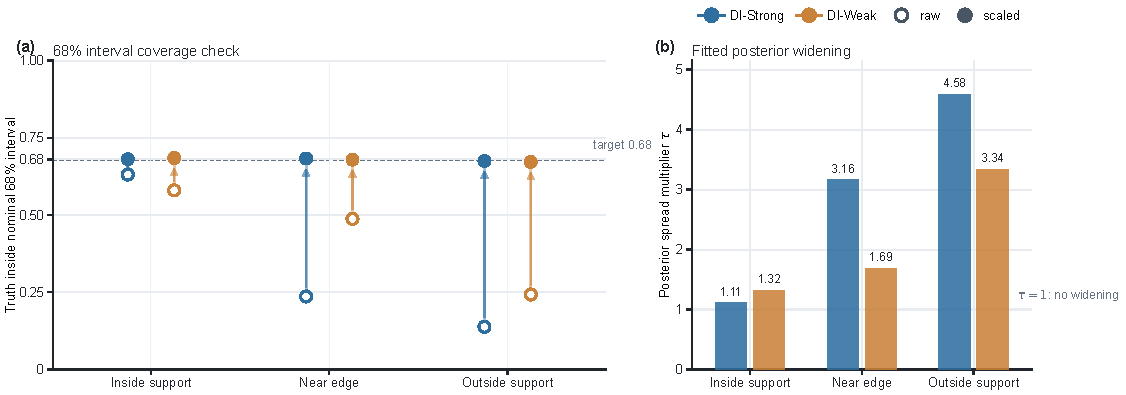
\includegraphics[width=\columnwidth]{figures/fig04_calibration_reliability_v4.pdf}
\caption{Split-sample posterior-temperature diagnostic for the matched production samplers. (a) Raw and temperature-scaled empirical coverage at the nominal 68 per cent interval level. (b) Posterior spread multiplier needed to bring the held-out mean coverage close to 0.68. Temperature scaling changes posterior spread around the median but does not change the posterior median or replace an observational-error model.}
\figalt{Two-panel calibration summary for DI-Strong and DI-Weak across inside-support, near-edge and outside-support regimes, showing raw and temperature-scaled 68 per cent coverage and fitted posterior spread multipliers.}
\label{fig:coverage}
\end{figure}

\subsection{Missing period bands and posterior uncertainty}

The production samplers were trained with intermittent-band mask augmentation to better match incomplete dispersion picks. We evaluate the fair weak-prior checkpoint on 1024 synthetic examples using fixed and random period windows (Fig.~\ref{fig:missingband}). Reducing the mean valid fraction from 0.351 for the nominal 2--60 s mask to 0.235 for the 2--40 s window increases $V_S$ MAE from 0.164 to 0.192 km s$^{-1}$ and increases mean $V_S$ posterior spread from 0.179 to 0.206 km s$^{-1}$. The narrower 10--30 s window is more restrictive, with valid fraction 0.135, $V_S$ MAE 0.276 km s$^{-1}$ and mean $V_S$ spread 0.287 km s$^{-1}$. The random-window experiment has mean width 29.8 s, valid fraction 0.187, $V_S$ MAE 0.208 km s$^{-1}$ and mean spread 0.221 km s$^{-1}$.

The random-window examples provide an internal consistency check: valid fraction is negatively correlated with both posterior spread ($r=-0.577$) and $V_S$ MAE ($r=-0.440$). In other words, the posterior becomes broader and less accurate when less period support is available. Coverage remains below nominal but comparatively stable across the window choices, with mean 16--84 per cent coverage between 0.615 and 0.646. Missing-band augmentation therefore improves robustness to incomplete inputs, but calibration and an observational-error model remain necessary for probability claims.

\begin{figure*}
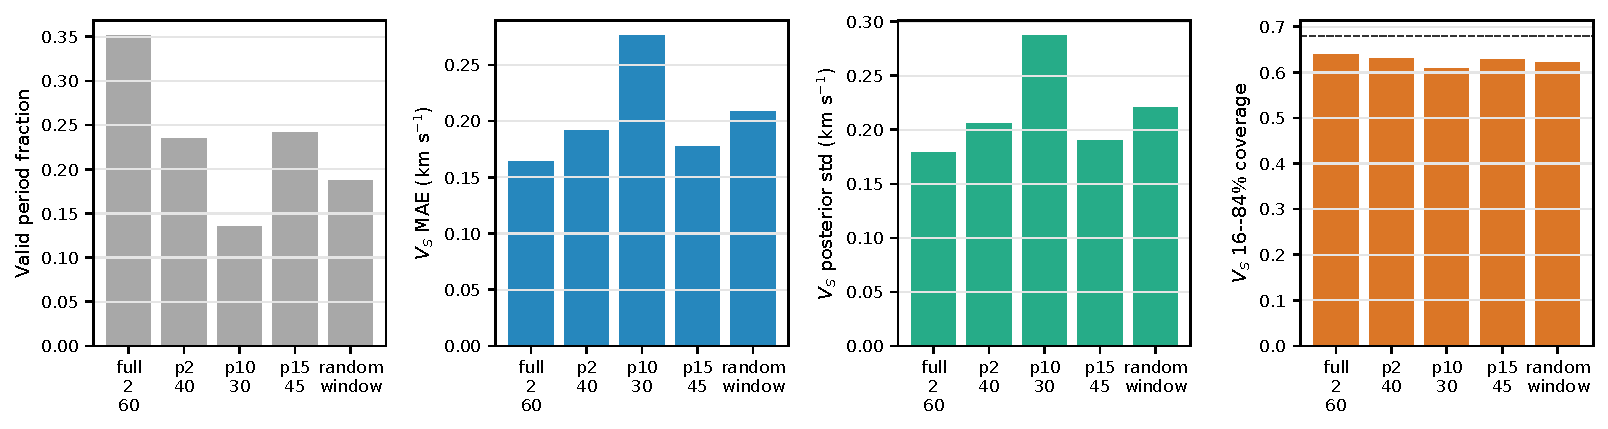
\includegraphics[width=0.48\textwidth]{figures/fair_missing_band_uncertainty.pdf}
\hfill
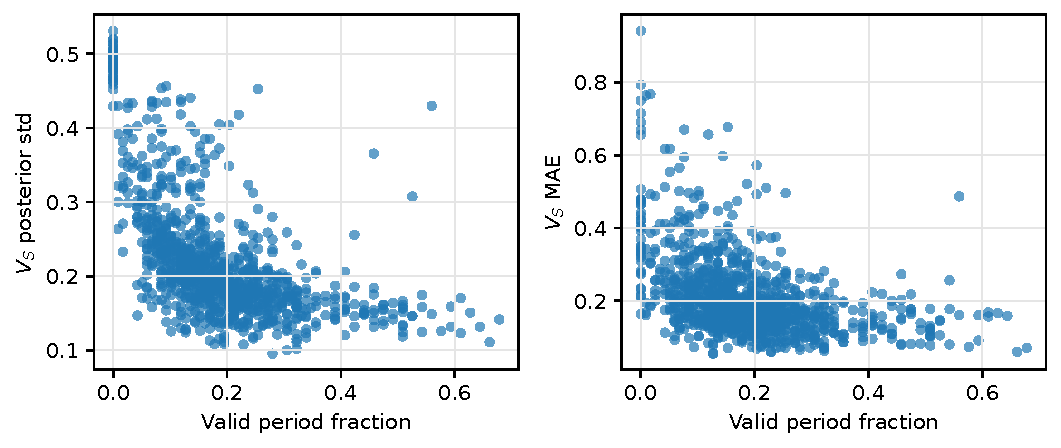
\includegraphics[width=0.48\textwidth]{figures/fair_missing_band_random_scatter.pdf}
\caption{Effect of missing period bands on weak-prior DNN posterior inversion. Left: fixed and random period-window diagnostics for posterior-median $V_S$ error, posterior spread and coverage. Right: random-window relationships between valid period fraction, posterior spread and error.}
\figalt{Bar charts and scatter plots showing that narrower or randomly incomplete period windows have lower valid-period fractions, larger shear-velocity errors and broader posterior spread.}
\label{fig:missingband}
\end{figure*}

\subsection{Evaluation-time phase-velocity noise}

The primary synthetic benchmark is mask-only, with no additive phase-velocity noise during training. We therefore treat additive noise as an evaluation-time sensitivity test rather than as a claim of noise-aware training (Fig.~\ref{fig:noise}). For inside-support DI-Weak, increasing Gaussian phase-velocity noise from 0 to 0.10 km s$^{-1}$ raises $V_S$ MAE from 0.133 to 0.299 km s$^{-1}$, raises mean posterior spread from 0.207 to 0.245, lowers mean raw coverage from 0.577 to 0.405 and increases the 68 per cent temperature factor from 1.336 to 2.053. DI-Strong shows the same trend, with inside-support $V_S$ MAE increasing from 0.086 to 0.199 km s$^{-1}$ and raw coverage falling from 0.638 to 0.394. This behaviour is expected: a sampler trained on a mask-only benchmark can recognise less consistent inputs through broader posterior summaries, but it has not learned a physical noise likelihood.

\begin{figure}

\includegraphics[width=\columnwidth]{figures/fair_noise_sensitivity.pdf}
\caption{Evaluation-time additive phase-velocity noise sensitivity. Gaussian noise is added only to observed Rayleigh/Love entries; masks and period channels are unchanged. The primary training condition remains the mask-only benchmark.}
\figalt{Line plots showing inside-support shear-velocity error, coverage, posterior standard deviation and temperature factor as additive phase-velocity noise increases from zero to 0.10 km per second.}
\label{fig:noise}
\end{figure}

\subsection{Prior support and reliability}

The prior-support experiment tests behaviour that is not visible from inside-support validation alone. It is a prior-support diagnostic rather than a final method ranking. DI-Weak reduces support-driven collapse near the strong-prior edge relative to DI-Strong (Table~\ref{tab:priorboundary}). Near-edge $V_S$ MAE decreases from 0.372 km s$^{-1}$ for DI-Strong to 0.171 km s$^{-1}$ for DI-Weak, and outside-support $V_S$ MAE decreases from 0.782 to 0.499 km s$^{-1}$. Dispersion residuals decrease from 0.277 to 0.100 km s$^{-1}$ for near-edge cases and from 0.335 to 0.262 km s$^{-1}$ for outside-support cases.

The pull-in statistic confirms that the improvement is a prior-support effect. For target values outside the strong-prior envelope, DI-Weak returns 0.101 of near-edge predictions and 0.318 of outside-support predictions inside that envelope, compared with 0.725 and 0.815 for DI-Strong. The comparison demonstrates that the learned posterior depends on prior width: a broader prior can reduce near-edge collapse, whereas the strong-prior control remains more accurate inside its own support.

\begin{table*}
\caption{Matched prior-support diagnostic for DI-Strong and DI-Weak trained from scratch with identical budgets. The table tests sensitivity to the training prior; it is not a general ranking of priors. Pull-in is the fraction of target values outside the strong-prior envelope whose posterior medians return inside that envelope. Bootstrap confidence intervals are reported in the full result tables.}
\label{tab:priorboundary}
\centering
\begin{tabular}{@{}llccccc@{}}
\toprule
Method & Regime & $N$ & $V_S$ MAE & Disp. MAE & $V_S$ coverage & Pull-in \\
 & & & (km s$^{-1}$) & (km s$^{-1}$) & & \\
\midrule
DI-Strong & Inside support & 1024 & 0.086 & 0.030 & 0.660 & 0.803 \\
DI-Strong & Near edge & 1024 & 0.372 & 0.277 & 0.250 & 0.725 \\
DI-Strong & Outside support & 1024 & 0.782 & 0.335 & 0.133 & 0.815 \\
DI-Weak & Inside support & 1024 & 0.134 & 0.049 & 0.786 & 0.706 \\
DI-Weak & Near edge & 1024 & 0.171 & 0.100 & 0.547 & 0.101 \\
DI-Weak & Outside support & 1024 & 0.499 & 0.262 & 0.264 & 0.318 \\
\bottomrule
\end{tabular}
\end{table*}

\subsection{Common-input comparison with QEDisp and DispFormer}

We next compare the DI samplers with a conventional inversion and a recent deterministic neural baseline on the same reference sites. The benchmark uses 128 CSRM sites from OpenSWI-real \citep{LiuEtAl2026OpenSWI}, the same 8--60 s Rayleigh fundamental-mode phase velocities, and the same CSRM reference $V_S$ profiles for all common-input methods. QEDispInv \citep{PanEtAl2026QEDispInv} is run as a fundamental-mode Rayleigh multistart inversion. DispFormer \citep{LiuEtAl2025DispFormer} is evaluated in two ways: a phase-only run that matches the common-input information, and its method-native phase+group run, which uses additional group-velocity input and is therefore shown separately.

The main result is that DI-Strong falls in the same point-error range as the conventional and deterministic neural baselines (Table~\ref{tab:commoninput}; Fig.~\ref{fig:commoninput}). The mean $V_S$ MAE is 0.108 km s$^{-1}$ for DI-Strong, compared with 0.104 km s$^{-1}$ for QEDisp fundamental-mode multistart inversion and 0.111 km s$^{-1}$ for DispFormer phase-only. DispFormer phase+group reaches 0.105 km s$^{-1}$ when group velocities are also supplied. DI-Weak is less accurate as a point estimator on this benchmark, with mean $V_S$ MAE of 0.138 km s$^{-1}$, but it returns broader posterior intervals. The important conclusion is therefore not that DI is more accurate than the baselines. It is that DI-Strong gives comparable point estimates while also returning posterior samples whose coverage and prior support can be checked.

\begin{table*}
\caption{Same-site CSRM benchmark. All common-input rows use Rayleigh fundamental-mode phase velocities between 8 and 60 s on the same 128 OpenSWI-real CSRM sites. DispFormer phase+group uses additional group velocities and is therefore included as a method-native reference rather than as a strict common-input comparison.}
\label{tab:commoninput}
\centering
\begin{tabular}{@{}p{0.30\textwidth}p{0.25\textwidth}cc@{}}
\toprule
Method & Input & Mean $V_S$ MAE & Median $V_S$ MAE \\
 & & (km s$^{-1}$) & (km s$^{-1}$) \\
\midrule
QEDisp multistart & Rayleigh phase & 0.104 & 0.100 \\
DI-Strong & Rayleigh phase & 0.108 & 0.106 \\
DI-Weak & Rayleigh phase & 0.138 & 0.128 \\
DispFormer phase-only & Rayleigh phase & 0.111 & 0.108 \\
DispFormer phase+group & Rayleigh phase + group & 0.105 & 0.101 \\
\bottomrule
\end{tabular}
\end{table*}

The mean best-fit Rayleigh dispersion RMS for QEDisp is 0.010 km s$^{-1}$. The mean forward-modelled Rayleigh phase RMS for DispFormer is 0.048 km s$^{-1}$ in the phase-only run and 0.035 km s$^{-1}$ in the phase+group run. For DI, the additional diagnostic is posterior coverage: the mean p05--p95 pointwise $V_S$ coverage against the CSRM reference is 0.680 for DI-Strong and 0.856 for DI-Weak.

\begin{figure*}
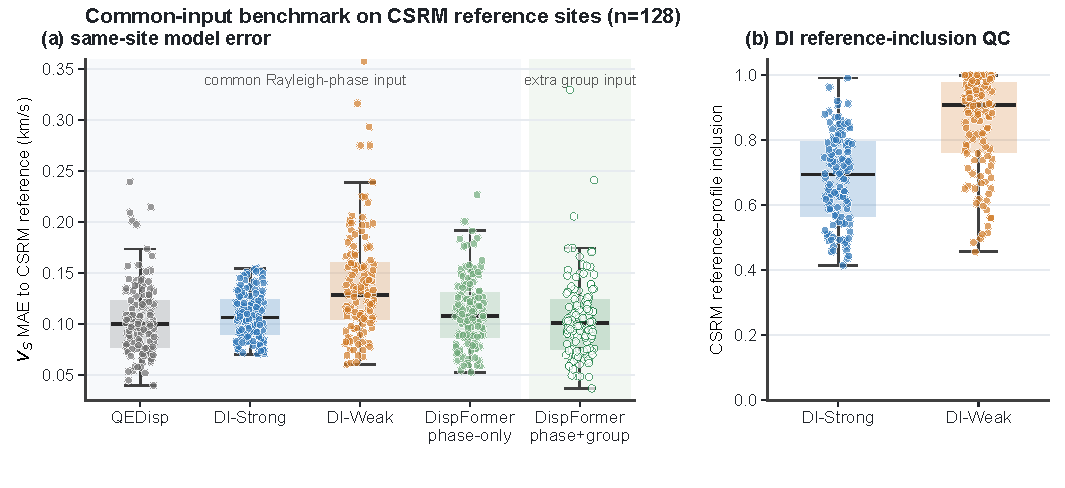
\includegraphics[width=\textwidth]{figures/fig05_common_input_benchmark.pdf}
\caption{Same-site CSRM common-input benchmark. (a) Distribution of $V_S$ MAE relative to the CSRM reference profile for QEDisp fundamental-mode multistart inversion, DI-Strong, DI-Weak, DispFormer phase-only and DispFormer phase+group. The first four methods use the same Rayleigh phase-velocity input; DispFormer phase+group uses additional group-velocity input and is shaded separately. (b) Empirical pointwise coverage of the CSRM reference profile by the DI p05--p95 posterior band. The dotted line marks the nominal 0.90 level.}
\figalt{Two-panel benchmark figure showing box-and-strip distributions of shear-velocity error for QEDisp, DI-Strong, DI-Weak and DispFormer on the same CSRM sites, plus posterior coverage for the two DI samplers.}
\label{fig:commoninput}
\end{figure*}

Representative site-level checks are shown in Fig.~\ref{fig:commonqc}. The dispersion panels show that several methods can match the Rayleigh phase observations closely even when their $V_S$ profiles differ at depth. This is expected for a non-unique surface-wave inverse problem and is the practical reason for reporting posterior ensembles rather than only a preferred profile.

\begin{figure*}
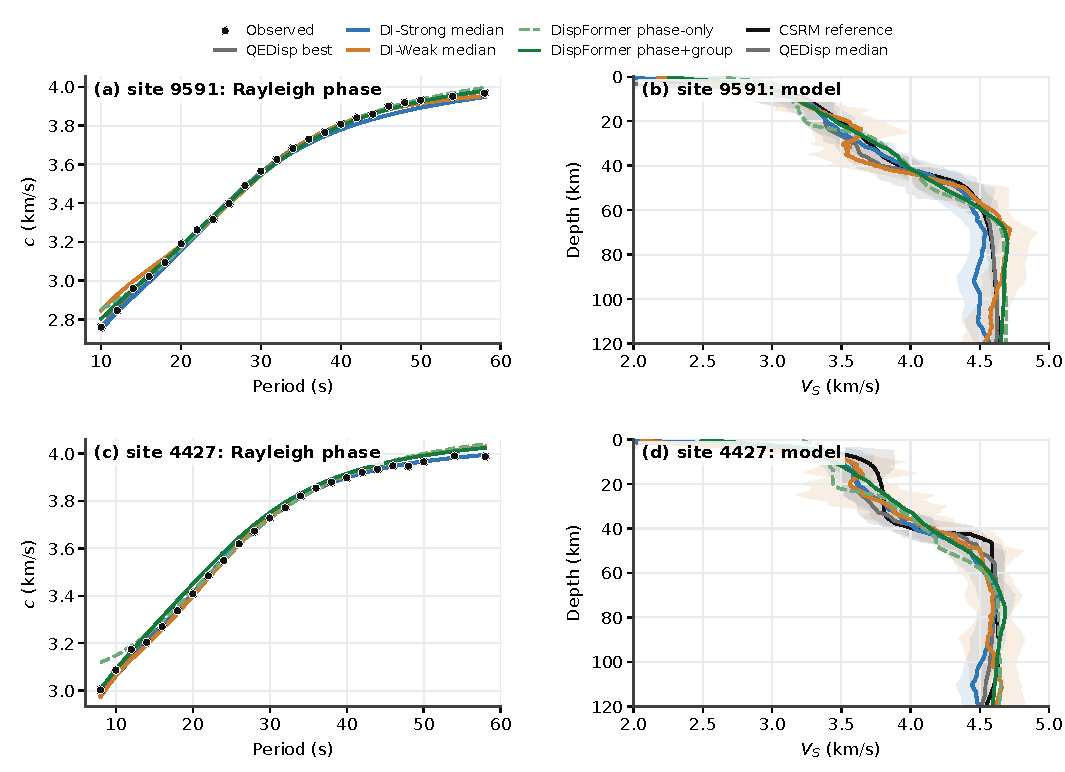
\includegraphics[width=\textwidth]{figures/fig06_common_input_qc_examples.pdf}
\caption{Representative same-site CSRM benchmark examples. Left panels show Rayleigh phase-velocity observations and forward-modelled curves from QEDisp, DI posterior medians and DispFormer predictions. Right panels show the corresponding $V_S$ profiles compared with the CSRM reference. Shaded DI bands are p05--p95 pointwise posterior intervals; the QEDisp band is its p10--p90 multistart interval. These examples are used as QC for the common-input benchmark, not as calibrated field-data posterior validation.}
\figalt{Four-panel QC figure with two CSRM sites. Each site has a Rayleigh phase-velocity fit panel and a shear-velocity profile panel comparing QEDisp, DI-Strong, DI-Weak and DispFormer with the CSRM reference.}
\label{fig:commonqc}
\end{figure*}

As an internal control, we also trained point-estimate DNN baselines with the same encoder, depth-control representation, structural priors and training budgets as the DI samplers. They reach similar inside-support point errors, for example $V_S$ MAE of 0.080 km s$^{-1}$ for the strong-prior point-estimate baseline and 0.127 km s$^{-1}$ for the weak-prior baseline. Their limitation is not point-estimate accuracy, but the absence of posterior samples, empirical interval coverage and posterior calibration diagnostics. The full internal baseline results are retained in the repository result tables rather than used as the main external comparison.

\section{Discussion}

\subsection{Relation to earlier probabilistic and pretrained inversions}

The present work builds on earlier Bayesian and neural probabilistic inversions. Classical Monte Carlo and transdimensional methods already provide posterior samples when a likelihood, prior and parameterisation are specified. Neural probabilistic methods have also been applied to surface-wave and related geophysical inversions, including probabilistic neural networks, mixture-density networks and invertible neural networks \citep{DevileeEtAl1999,MeierEtAl2007,EarpEtAl2020,ZhangCurtis2021,KeilWassermann2023,YablokovEtAl2023}. Those studies establish that learned methods can approximate uncertain inverse solutions at much lower inference cost than repeated conventional sampling.

Our emphasis is on the audit of the learned posterior. We treat it as a conditional distribution defined by a synthetic prior-predictive experiment, and then ask how that distribution should be checked. The matched DI-Strong/DI-Weak comparison tests prior support directly; the reliability curves, depth-binned coverage, rank diagnostics and posterior-temperature scaling test calibration; the missing-band and noise experiments test robustness to common observation changes; and the QEDisp/DispFormer comparison keeps point-estimate performance in view. This framing is deliberately narrower than recent pretrained or variable-period approaches such as DispFormer, but it addresses a different need: making learned posterior probabilities auditable before they are used as geophysical uncertainty.

As a small posterior anchor, Appendix Fig.~\ref{fig:mcmcanchorinside} compares DI-Strong with a reduced prior-matched MCMC reference on synthetic cases. The comparison is not an exact full-dimensional Bayesian solution for the procedural generator, but it checks whether the learned sampler gives similar medians and intervals when the parameterisation, prior approximation, forward solver, mask and error scale are matched as closely as practical.

\subsection{Meaning of DNN posterior probability}

The DNN posterior is not a property of the dispersion curve alone. It is conditioned by the synthetic model generator, the forward solver, the observation mask, the noise model and the depth-control basis. This is a strength when those ingredients represent the intended inversion problem: once trained, the sampler provides fast posterior draws, uncertainty summaries and posterior-predictive checks. It is also a limitation. Changing the structural generator, forward solver, masking process, observational-error model or depth basis changes the distribution being learned.

This interpretation is important for field use. The DNN does not learn an assumption-free inverse map. It learns to sample models for the synthetic distribution used in training. Posterior samples are therefore meaningful only together with the prior, mask, noise assumption and parameterisation that produced the training data. These choices should be reported as part of the method, not hidden as data-generation details.

\subsection{Posterior uncertainty and calibration}

Posterior ensembles allow uncertainty summaries that deterministic DNN inversion cannot provide directly: medians, pointwise credible intervals, posterior standard deviations, posterior density views and posterior-predictive checks. These summaries are nevertheless not automatically calibrated Bayesian probabilities. Raw DNN intervals can under-cover the held-out synthetic truth, meaning that the true model falls outside nominal credible intervals too often. If uncorrected, this would make the posterior ensemble look more certain than it is.

The scalar temperature diagnostic is a simple empirical correction of posterior dispersion. It widens or narrows the sampled ensemble around the posterior median to improve held-out coverage, but it is not a physical likelihood model and does not replace an observational-error model. Field dispersion picks have frequency-dependent uncertainty, inter-period covariance, processing bias and wave-type differences. A field posterior should include those errors in $p_\epsilon$ or in a likelihood-tempering scheme and should be checked against independent posterior calculations, repeat measurements or trusted reference models.

The same caution applies to posterior-predictive checks. A posterior draw can be forward-modelled to test whether it reproduces observed dispersion, but the interpretation of residuals depends on the observational error model. Without it, a small residual is only consistency with the encoded observation vector, not proof of a unique or calibrated Earth model.

\subsection{Prior support as a reliability check}

The prior-support diagnostic shows how a learned posterior can fail outside the support of its training distribution. Strong-prior near-edge collapse is not merely an architecture failure. It is the expected result of training a fast sampler under a restricted prior. The weak-prior comparison confirms this interpretation: changing the prior changes posterior behaviour in the predicted direction.

The correct message is not that weak priors are always better. A weak prior is useful when structural support is uncertain, because it is less likely to exclude plausible models before seeing the data. Geology-guided priors are valuable when they are independently justified by mapping, boreholes, receiver functions, active-source constraints or preliminary inversions. The strong prior used here is therefore not an artificial negative control; it is a useful production-scale architecture and calibration baseline within its own prior support. The comparison demonstrates that prior support must be explicit, tested and calibrated.

\subsection{Parameterisation and prior design}

The depth-control basis improves sample regularity and reduces high-frequency artefacts, but it also restricts model space. This is analogous to layer-count, spline, Voronoi or transdimensional choices in conventional Bayesian surface-wave inversion \citep{GaoLekic2018}. A posterior interval produced under one basis should not be interpreted as basis-independent uncertainty. Thin low-velocity layers, sharp discontinuities or complex sedimentary structures may require different controls, hierarchical basis selection or targeted prior enrichment.

Explicit geological parameterisations can improve recovery of interfaces, faults and localised anomalies when such structures are supported by mapping, boreholes or preliminary inversions. This is complementary to the present work. The current manuscript focuses on probabilistic DNN posterior sampling and uncertainty calibration; future work could combine conditional-flow posterior sampling with interface-aware or level-set geological priors.

\subsection{Implications for field or regional use}

Many practical studies assemble local or path-averaged 1-D inversions into maps or 3-D volumes. Repeated near-edge prior bias can therefore become a coherent regional artefact, such as clipped Moho depth, suppressed low-velocity-zone amplitude or overly prior-typical upper-mantle $V_S$. A DNN posterior inversion should therefore be used with prior-support diagnostics, posterior-predictive checks, calibration sets and transparent reporting of the synthetic prior. The speed of the trained sampler is most valuable when paired with these checks, because thousands of local posterior ensembles can be generated and checked quickly.

\subsection{Limitations and future work}

The present fair comparison removes the training-budget difference between DI-Strong and DI-Weak, but it is still a single-seed synthetic benchmark. The reported checks include bootstrap intervals, depth-binned coverage, reliability curves, rank/PIT diagnostics, missing-band tests, additive-noise sensitivity, posterior-predictive dispersion residuals, deterministic DNN baselines, sampling-step sensitivity checks and a same-site CSRM comparison with QEDisp and DispFormer. They do not include a calibrated field-data posterior validation. Field-facing extensions should add multiple random seeds, noise-aware or likelihood-aware training, a field-specific observational-error model, period bands matched to the target observations and independent calibration or reference constraints. These additions would extend the same central message: DNN posterior estimates should be sampled, calibrated and audited rather than treated as unchecked point predictions.

\section{Conclusions}

We formulated surface-wave dispersion inversion as probabilistic direct inversion using a depth-controlled conditional rectified flow. The main methodological result is an audited learned posterior sampler: a network trained on synthetic model--dispersion pairs can sample $q_\theta({\bf m}|{\bf d})$ for the stated synthetic inversion problem, and the resulting ensemble can be checked with posterior-predictive tests, empirical coverage, calibration diagnostics and prior-support tests.

The matched production runs test the architecture, depth-control basis and calibration diagnostics under two structural priors. On the inside-support diagnostic, DI-Strong reaches $V_S$ MAE of 0.086 km s$^{-1}$ and mean 16--84 per cent pointwise coverage of 0.638, while DI-Weak reaches 0.134 km s$^{-1}$ and 0.577. Empirical coverage, missing-band stress tests, additive-noise sensitivity and posterior-temperature scaling provide practical diagnostics for uncertainty calibration, while also showing that raw DNN interval widths should not be accepted without checking.

On the same-site CSRM common-input benchmark, DI-Strong reaches mean $V_S$ MAE of 0.108 km s$^{-1}$ using Rayleigh phase velocities alone, comparable to QEDisp fundamental-mode multistart inversion (0.104 km s$^{-1}$) and DispFormer phase-only prediction (0.111 km s$^{-1}$). DispFormer phase+group reaches 0.105 km s$^{-1}$ when group velocities are also supplied. This comparison supports a conservative claim: the proposed sampler is competitive as a point estimator, but its main value is the posterior ensemble and the ability to audit coverage, prior support and posterior-predictive consistency.

The prior-support experiment shows that posterior uncertainty must be interpreted under the training prior. In the matched $N=1024$ diagnostic, DI-Weak reduces near-edge and outside-support $V_S$ errors to 0.171 and 0.499 km s$^{-1}$ and lowers pull-in fractions relative to the strong-prior control. DI-Strong remains more accurate inside its own training prior, with inside-support $V_S$ MAE of 0.086 km s$^{-1}$ compared with 0.134 km s$^{-1}$ for DI-Weak, but it degrades to 0.372 km s$^{-1}$ near the edge and 0.782 km s$^{-1}$ outside support. This is a test of training-prior support, not a general ranking of priors. Field use requires explicit observational-error modelling, empirical calibration and prior-support checks.

The current sampler is therefore a controlled probabilistic inversion framework rather than a general-purpose surface-wave foundation model. Future work should extend the same posterior-audit philosophy to variable-period inputs, broader wave-type combinations, field-specific error models, matched-period field calibration data and independently justified geological constraints.

\section*{Acknowledgments}

The authors thank the developers of Python, PyTorch, matplotlib, disba and Computer Programs in Seismology.

\section*{AI-use disclosure}

OpenAI Codex was used for editorial assistance with manuscript restructuring, LaTeX consistency checks, figure-inclusion auditing and drafting of a cover-letter disclosure. All scientific claims, code, data, citations and numerical results were checked by the authors. No numerical result, citation, data source or DOI was generated by AI without author verification.

\section*{Conflict of Interest}

The authors declare no competing interests.

\begin{dataavailability}
\noindent\textbf{Data Availability and Software Availability.}
The code, synthetic-data generators, configs, random seeds, plotting scripts, evaluation CSV/JSON outputs and manuscript build commands used for this version are available in the project repository at \url{https://github.com/cangyeone/SurfFlow}. The CSRM same-site benchmark uses the OpenSWI-real data product \citep{LiuEtAl2026OpenSWI}. External baseline calculations use QEDispInv \citep{PanEtAl2026QEDispInv} and DispFormer \citep{LiuEtAl2025DispFormer}; the wrapper scripts and extracted benchmark tables used for the comparisons are archived with the SurfFlow result files. Checkpoint identifiers, training metadata and exact evaluation commands are recorded in the repository README files and result-table protocols. Because GitHub is not used here for large binary files, model weights and large diagnostic arrays need to be supplied through a separate archive for final submission, or regenerated from the recorded training commands.
\end{dataavailability}

\clearpage

\bibliographystyle{gji}
\bibliography{references}

\appendix
\setcounter{table}{0}
\renewcommand{\thetable}{A\arabic{table}}
\renewcommand{\theHtable}{A\arabic{table}}
\setcounter{figure}{0}
\renewcommand{\thefigure}{A\arabic{figure}}
\renewcommand{\theHfigure}{A\arabic{figure}}

\section{Synthetic generators, training configuration and evaluation protocol}

\subsection{Synthetic generator and observation protocol}

Table~\ref{tab:generatorprotocol} records the synthetic assumptions used by the present manuscript. These choices define the distribution learned by the DNN; changing any of them changes the resulting posterior samples.

\small
\begin{longtable}{@{}p{0.24\textwidth}p{0.66\textwidth}@{}}
\caption{Synthetic generator and observation protocol used in the present manuscript. Additional generator constants are defined in the repository-local scripts and result metadata.}
\label{tab:generatorprotocol}\\
\toprule
Item & Current manuscript setting \\
\midrule
\endfirsthead
\caption[]{Synthetic generator and observation protocol used in the present manuscript (continued).}\\
\toprule
Item & Current manuscript setting \\
\midrule
\endhead
\bottomrule
\endfoot
Strong structural generator & Five tectonic classes: oceanic, shield, platform, orogen and rift. Class-dependent ranges set sediment thickness, Moho depth, crustal and mantle $V_S$, and low-velocity-zone probability, depth and amplitude. $V_P$ is generated from layer-dependent $V_P/V_S$ ratios and density from empirical relations. \\
Weak structural generator & Broad depth-dependent bounds without explicit tectonic class labels, Moho templates or prescribed low-velocity-zone forms. Profiles are generated from random smooth controls, broad $V_S$ ranges, clipped $V_P/V_S$ ratios and physical constraints including $V_P>V_S$ and positive density. \\
Depth grid & Regular 0.5 km grid. The network and metrics use the first 256 nodes, representing 0--127.5 km. \\
Dispersion periods & Fundamental-mode Rayleigh and Love phase velocities from 2 to 60 s at 1 s spacing, giving 59 period samples. \\
Forward solver & Python surface-wave forward calculations based on Computer Programs in Seismology (CPS) through the \texttt{disba}/CPS implementation used by the repository scripts. Failed synthetic forward attempts are retried during dataset generation. \\
Observation encoding & Five channels: normalised period, Rayleigh phase velocity, Love phase velocity, Rayleigh mask and Love mask. Missing velocities are zero-filled after normalisation and identified by masks. \\
Mask distribution & The reported sampler uses intermittent-band mask augmentation. Preset windows include 2--40, 10--30, 5--35 and 15--45 s; random windows span 15--45 s, can contain up to six internal holes and include a small point-drop probability. The generator includes Rayleigh-only, Love-only and both-wave cases. \\
Synthetic noise & Mask-only synthetic benchmark with no additive phase-velocity noise. In eq.~\eqref{eq:priorpredictive}, $p_\epsilon$ is therefore a point mass at zero for the experiments reported here; field-facing use requires an explicit observational-error model. \\
Normalisation & Model and dispersion normalisation statistics are estimated from the training distribution and stored with the checkpoints. Exported means and scales are listed in the repository metadata. \\
\end{longtable}
\normalsize

\small
\begin{longtable}{@{}p{0.22\textwidth}p{0.34\textwidth}p{0.34\textwidth}@{}}
\caption{Main structural-prior parameters used by the matched DI-Strong and DI-Weak generators. Values are taken from the repository generator scripts used for the production runs. The weak prior is still a prior: it uses broad bounds, smoothing and physical consistency constraints, but it avoids explicit tectonic classes and Moho/LVZ templates.}
\label{tab:priorparameters}\\
\toprule
Parameter & DI-Strong generator & DI-Weak generator \\
\midrule
\endfirsthead
\caption[]{Main structural-prior parameters used by the matched DI-Strong and DI-Weak generators (continued).}\\
\toprule
Parameter & DI-Strong generator & DI-Weak generator \\
\midrule
\endhead
\bottomrule
\endfoot
Structural organization & Five tectonic classes: oceanic, shield, platform, orogen and rift. & No tectonic class labels; random smooth knots and correlated perturbations under depth-dependent bounds. \\
Crustal thickness or Moho control & Class-dependent crustal-thickness ranges: 5--15, 20--40, 28--45, 35--55 and 40--70 km across the five classes. & No explicit Moho parameter or layer template. \\
Sediment thickness & Class-dependent ranges from 0--3 km to 1--12 km. & No explicit sediment-thickness parameter; shallow low velocities are allowed by the broad near-surface $V_S$ envelope. \\
$V_S$ support & Layer- and class-dependent ranges. Sediment $V_S$ spans 0.2--3.0 km s$^{-1}$ across classes; upper crust 2.6--3.9 km s$^{-1}$; lower crust 3.2--4.4 km s$^{-1}$; upper mantle 4.0--5.2 km s$^{-1}$. & Piecewise linear broad envelope: lower bound 0.15, 0.25, 1.5, 2.5, 3.0, 3.6 and 3.8 km s$^{-1}$ at 0, 3, 8, 20, 40, 80 and 150 km; upper bound 4.0, 4.2, 4.5, 4.8, 5.1, 5.4 and 5.6 km s$^{-1}$. \\
Low-velocity-zone structure & Explicit class-dependent LVZ probability 0.3--0.85; centre depth ranges 50--140 km, thickness ranges 30--80 km and amplitude ranges 3--15 per cent depending on class. & No explicit LVZ template; broad random knots and Gaussian perturbations can generate positive or negative smooth anomalies. \\
$V_P/V_S$ and $V_P$ & Layer-dependent truncated $V_P/V_S$ ratios with class-specific means; density from the Brocher relation. & Smooth depth-dependent $V_P/V_S$ profile clipped to 1.65--2.00; $V_P$ clipped to 1.0--12.5 km s$^{-1}$ and density clipped to 1.0--3.8 g cm$^{-3}$. \\
Random variability and smoothing & Layer gradients, pointwise Gaussian perturbations, smoothing and monotonicity checks inside the class template. & 6--12 random knots, depth-dependent perturbation standard deviation 0.20--0.10 km s$^{-1}$ from surface to 150 km, correlation length 2--18 km and additional Gaussian anomalies with amplitude up to 0.35 km s$^{-1}$. \\
\end{longtable}
\normalsize

\subsection{Training and evaluation protocol}

\small
\begin{longtable}{@{}p{0.24\textwidth}p{0.66\textwidth}@{}}
\caption{Training and evaluation protocol for the matched strong- and weak-prior production comparison.}
\label{tab:trainingprotocol}\\
\toprule
Item & Current manuscript setting \\
\midrule
\endfirsthead
\caption[]{Training and evaluation protocol for the matched strong- and weak-prior production comparison (continued).}\\
\toprule
Item & Current manuscript setting \\
\midrule
\endhead
\bottomrule
\endfoot
Architecture & One-dimensional residual convolutional encoder with five input channels and a 256-dimensional conditioning vector; conditional rectified-flow MLP in depth-control space with 28 controls for each of $V_P$, $V_S$ and density. The logged production model has approximately 4.26 million trainable parameters. \\
Depth controls & 28 controls, dense near the surface and coarser at depth: 0--5 km every 0.5 km, 5--10 km every 1 km, 10--50 km every 5 km and 50--127.5 km every 20 km, with endpoints included. \\
Loss function & SmoothL1 rectified-flow velocity loss plus a one-step reconstruction term and small first- and second-difference penalties after interpolation to the full depth grid. \\
Strong-prior training & Trained from scratch with 100000 synthetic profiles, 2048 validation profiles, batch size 64, 24 scheduled epochs and seed 642026. The selected checkpoint is the best-validation checkpoint. \\
Weak-prior training & Trained from scratch with the same architecture, optimizer, learning-rate schedule, batch size, train/validation sizes, epochs, loss weights, mask augmentation and seed as DI-Strong. The only intended difference is the structural prior generator. The selected checkpoint is the best-validation checkpoint. \\
Optimisation & AdamW with cosine learning-rate scheduling and gradient clipping in the repository training script. Optimiser hyperparameters are listed in the repository metadata. \\
Posterior sampling & Synthetic posterior summaries use 64 samples and 24 Euler integration steps. \\
Evaluation sizes & The matched DI comparison uses $N=1024$ examples per inside-support, near-edge and outside-support regime. The prior envelope uses $N=10000$. The missing-band and additive-noise diagnostics use $N=1024$. The deterministic DNN baselines use $N=1024$ per regime; the learned-forward optimisation baseline uses a smaller $N=128$ reference set. \\
Calibration & Scalar posterior-temperature scaling is fitted on 1024 calibration examples and evaluated on 1024 held-out examples for each method and regime. Reliability curves, rank diagnostics and depth-binned coverage are exported in the production result archive. Bootstrap intervals use 2000 resamples for the matched DI comparison tables. \\
Field-facing scope & No calibrated field-data inversion is used as evidence in this manuscript. Field deployment requires observations whose period band matches the training/evaluation problem, an explicit observational-error model and independent calibration or reference data. \\
\end{longtable}
\normalsize

\subsection{Reduced prior-matched MCMC posterior anchor}

To check the learned posterior against a conventional sampling reference, we ran a reduced prior-matched MCMC calculation for a small set of synthetic examples. The reference samples $V_S$ at 10 depth knots (0, 2, 5, 10, 20, 35, 50, 75, 100 and 127.5 km) and one median $V_P/V_S$ parameter. A full-covariance Gaussian-mixture prior is fitted to 2500 projections from the DI-Strong synthetic generator. The forward model, Rayleigh/Love fundamental-mode mask and period grid match the DI examples, while the likelihood uses an independent Gaussian phase-velocity error scale of 0.10 km s$^{-1}$. This construction is a reduced Bayesian reference, not the exact full posterior of the original procedural Earth generator; remaining DI--MCMC differences can therefore reflect neural approximation error, reduced parameterisation and prior-approximation mismatch.

Inside the synthetic support, the DI-Strong posterior medians and p05--p95 bands are broadly consistent with the MCMC reference (Fig.~\ref{fig:mcmcanchorinside}). Across six validated inside-support cases, the mean DI--MCMC median $V_S$ difference is 0.057 km s$^{-1}$, the mean p05--p95 interval overlap is 0.58 and the mean DI/MCMC interval-width ratio is 1.21. Near and outside the support, the same comparison becomes less stable (Fig.~\ref{fig:mcmcanchortransition}), which reinforces the main prior-support message of the paper.

\begin{figure*}

\includegraphics[width=\textwidth]{figures/mcmc_anchor_inside_support_profiles.pdf}
\caption{Reduced prior-matched MCMC posterior anchor for six inside-support synthetic cases. The MCMC reference uses a 10-knot $V_S$ parameterisation and a Gaussian-mixture prior fitted to projections from the DI-Strong synthetic prior. Lines show posterior medians and shaded bands show pointwise p05--p95 intervals. Inside the synthetic support, DI-Strong gives similar median profiles and comparable interval widths to this reduced Bayesian reference.}
\figalt{Six shear-velocity profile panels comparing target profiles, MCMC medians and p05--p95 intervals, and DI-Strong medians and p05--p95 intervals for inside-support synthetic examples.}
\label{fig:mcmcanchorinside}
\end{figure*}

\begin{figure*}

\includegraphics[width=\textwidth]{figures/mcmc_anchor_support_transition_profiles.pdf}
\caption{Reduced prior-matched MCMC anchor across prior-support regimes. The inside-support case shows close DI--MCMC agreement. The near-edge and outside-support cases show larger differences between the learned posterior and the reduced MCMC reference, even when the posterior-predictive fit remains acceptable. This is why the posterior is interpreted together with prior-support, coverage and posterior-predictive diagnostics rather than as an unchecked Bayesian probability.}
\figalt{Three shear-velocity profile panels comparing target profiles, MCMC posterior medians and intervals, DI posterior medians and intervals, and the projected prior interval for inside-support, near-edge and outside-support cases.}
\label{fig:mcmcanchortransition}
\end{figure*}

\subsection{Calibration and sampling-sensitivity diagnostics}

Table~\ref{tab:calibrationappendix} summarizes the depth-binned and rank/probability-integral-transform (PIT) diagnostics exported by the calibration script. The rank/PIT edge mass is the fraction of rank values in the two outermost 5 per cent bins; a uniform diagnostic would have an edge mass of 0.10. Table~\ref{tab:samplingsensitivity} reports a lightweight DI-Weak sensitivity check on $N=128$ inside-support and near-edge examples. It is not used as a method-ranking table, but it verifies that the reported conclusions are not tied to a single arbitrary sample count or Euler-step setting.

\small
\begin{longtable}{@{}llccccc@{}}
\caption{Calibration diagnostic summary from the production held-out split. Raw and temperature-scaled columns report mean pointwise 68 per cent coverage. The depth-binned range is the raw 68 per cent coverage range over channel-depth bins, and edge mass reports rank/PIT non-uniformity in the raw posterior.}
\label{tab:calibrationappendix}\\
\toprule
Method & Regime & Raw cov. & Scaled cov. & $\tau$ & Depth-bin range & Rank edge mass \\
\midrule
\endfirsthead
\caption[]{Calibration diagnostic summary from the production held-out split (continued).}\\
\toprule
Method & Regime & Raw cov. & Scaled cov. & $\tau$ & Depth-bin range & Rank edge mass \\
\midrule
\endhead
\bottomrule
\endfoot
DI-Strong & Inside support & 0.631 & 0.681 & 1.11 & 0.588--0.752 & 0.201 \\
DI-Strong & Near edge & 0.236 & 0.683 & 3.16 & 0.076--0.601 & 0.638 \\
DI-Strong & Outside support & 0.138 & 0.675 & 4.58 & 0.041--0.573 & 0.799 \\
DI-Weak & Inside support & 0.580 & 0.685 & 1.32 & 0.205--0.860 & 0.281 \\
DI-Weak & Near edge & 0.488 & 0.679 & 1.69 & 0.336--0.719 & 0.368 \\
DI-Weak & Outside support & 0.243 & 0.672 & 3.34 & 0.152--0.405 & 0.661 \\
\end{longtable}
\normalsize

\small
\begin{longtable}{@{}llcccccc@{}}
\caption{DI-Weak posterior sample-count and Euler-step sensitivity check. Metrics are computed on $N=128$ examples per regime using the matched weak-prior checkpoint. Runtime is wall-clock sampling time on the local MPS device and excludes one-time data generation and model loading.}
\label{tab:samplingsensitivity}\\
\toprule
Regime & Samples & Steps & $V_S$ MAE & Coverage & $V_S$ std & Disp. MAE & Runtime \\
 & & & (km s$^{-1}$) & & (km s$^{-1}$) & (km s$^{-1}$) & (s) \\
\midrule
\endfirsthead
\caption[]{DI-Weak posterior sample-count and Euler-step sensitivity check (continued).}\\
\toprule
Regime & Samples & Steps & $V_S$ MAE & Coverage & $V_S$ std & Disp. MAE & Runtime \\
 & & & (km s$^{-1}$) & & (km s$^{-1}$) & (km s$^{-1}$) & (s) \\
\midrule
\endhead
\bottomrule
\endfoot
Inside support & 16 & 12 & 0.135 & 0.518 & 0.184 & 0.055 & 2.9 \\
Inside support & 16 & 24 & 0.134 & 0.533 & 0.190 & 0.051 & 2.7 \\
Inside support & 16 & 48 & 0.136 & 0.543 & 0.194 & 0.053 & 3.4 \\
Inside support & 32 & 12 & 0.131 & 0.548 & 0.188 & 0.048 & 4.6 \\
Inside support & 32 & 24 & 0.131 & 0.559 & 0.196 & 0.047 & 5.4 \\
Inside support & 32 & 48 & 0.133 & 0.572 & 0.200 & 0.051 & 6.6 \\
Inside support & 64 & 12 & 0.131 & 0.560 & 0.189 & 0.047 & 8.8 \\
Inside support & 64 & 24 & 0.128 & 0.577 & 0.196 & 0.048 & 10.7 \\
Inside support & 64 & 48 & 0.129 & 0.586 & 0.203 & 0.048 & 12.7 \\
Inside support & 128 & 12 & 0.128 & 0.573 & 0.191 & 0.048 & 18.3 \\
Inside support & 128 & 24 & 0.128 & 0.583 & 0.198 & 0.049 & 23.5 \\
Inside support & 128 & 48 & 0.128 & 0.591 & 0.202 & 0.047 & 31.2 \\
Near edge & 16 & 12 & 0.166 & 0.438 & 0.137 & 0.096 & 2.5 \\
Near edge & 16 & 24 & 0.166 & 0.448 & 0.141 & 0.098 & 3.0 \\
Near edge & 16 & 48 & 0.168 & 0.462 & 0.145 & 0.099 & 3.7 \\
Near edge & 32 & 12 & 0.165 & 0.462 & 0.139 & 0.096 & 5.5 \\
Near edge & 32 & 24 & 0.162 & 0.477 & 0.144 & 0.096 & 6.2 \\
Near edge & 32 & 48 & 0.166 & 0.483 & 0.149 & 0.097 & 7.4 \\
Near edge & 64 & 12 & 0.163 & 0.476 & 0.141 & 0.095 & 11.4 \\
Near edge & 64 & 24 & 0.164 & 0.493 & 0.147 & 0.096 & 17.0 \\
Near edge & 64 & 48 & 0.162 & 0.497 & 0.150 & 0.097 & 14.9 \\
Near edge & 128 & 12 & 0.161 & 0.481 & 0.142 & 0.095 & 22.1 \\
Near edge & 128 & 24 & 0.162 & 0.496 & 0.148 & 0.096 & 25.4 \\
Near edge & 128 & 48 & 0.162 & 0.504 & 0.150 & 0.096 & 28.4 \\
\end{longtable}
\normalsize

\label{lastpage}
\end{document}
